\documentclass[11pt,twoside,a4paper]{cernrep}
\usepackage{fcc_common}
\usepackage{amssymb}
\usepackage[final]{epsfig}
\usepackage{color}
\usepackage{xcolor}
\usepackage{graphicx}
\usepackage{lineno}
\usepackage{verbatim}
%\usepackage{natbib}
%\newcommand{\textmu}{$\mu$}
%\newcommand{\textnu}{$\nu$}
%\newcommand{\texttau}{$\tau$}
%\newcommand{\textgamma}{$\gamma$}
\newcommand{\hl}{}
%\newcommand{\textpi}{$\pi$}
\newcommand*{\effg}{\ensuremath{\epsilon_{\gamma}}}
\newcommand*{\misg}{\ensuremath{\epsilon_{j \rightarrow \gamma}}}
\newcommand*{\effb}{\ensuremath{\epsilon_{b}}}
\newcommand*{\misl}{\ensuremath{\epsilon_{l \rightarrow b}}}
\newcommand*{\misc}{\ensuremath{\epsilon_{c \rightarrow b}}}
\newcommand*{\mislc}{\ensuremath{\epsilon_{l(c) \rightarrow b}}}
\newcommand*{\maa}{\ensuremath{m_{\gamma\gamma}}}
\newcommand*{\mbb}{\ensuremath{m_{bb}}}

\newcommand{\MS}[1]{\textbf{\textcolor{purple}{MS - #1}}}
\newcommand{\MLM}[1]{\textbf{\textcolor{blue}{MLM - #1}}}
\newcommand{\CH}[1]{\textbf{\textcolor{green}{CH - #1}}}



\begin{document}
%%%%%%%%%%%%%%%%%%%%%%%%%%%%%%%%%%%%%%%%%%%%%%%%%%%%%%%%%%%%%%%%%
%%%%%%%%%%%%%%%%%%%%%%%%%%%%%%%%%%%%%%%%%%%%%%%%%%%%%%%%%%%%%%%%%

\section{Detector Performance and Physics Benchmark Studies}

Physics at the FCC-hh will involve final states particles with momenta ranging from a few tens of GeV to tens of TeV. The high end of the spectrum features searches for resonances at the highest possible mass (up to 40 TeV), whose decay products are SM multi-TeV particles. High momentum decay products such as muons, electrons, photons or charged hadrons can be used to define minimal requirements on tracking and calorimetry momentum/energy resolution. Multi-TeV unstable heavy objects such as gauge bosons, top or bottom quarks and tau leptons that decay into highly boosted and collimated stable particles are instead useful benchmarks for constraining the angular separation power of the detector, in particular of the tracker and of the calorimeters. At such high $p_{T}$ the relative impact of pile-up can be neglected as a first approximation, as shown in Figures~\ref{ecal_electronics_noise}a and~\ref{hcal}a \MS{make sure proper referencing is made}. The detector performance at low $p_{T}$ is instead fixed by targeting maximal precision and by requiring the best sensitivity to searches for elusive final states, such as those involving compressed or low-mass spectra. The goal is to define targets for object reconstruction efficiencies and fake-rates, as well as energy/momentum resolution at low momentum, in a regime where the relative impact of the pile-up is large.

A complete discussion of the physics opportunities at the FCC-hh can be found in Volume~1. In this section we focus on a small selection of physics studies, which played a key role in defining the target performance for the FCC-hh baseline detector presented in the previous sections and in shaping its design. We start by presenting the measurement of the Higgs self-coupling, and the impact of pile-up. We cover next the search for a Z$^{\prime}$ resonance decaying to leptons, and for a pair of stop squarks decaying to fully hadronic final states. These searches define the momentum resolution and calorimeter granularity requirements for multi-TeV leptons and boosted hadronic jets, respectively. Finally, we present a search for \emph{disappearing tracks}, with a focus on the inner tracking detector design. A more complete description of those analyses can be found in the following documents~\cite{Selvaggi:2642471,Helsens:2642473,Gouskos:2642475,Terashi:2642474}.

For the studies presented in this section, most of the Monte Carlo samples have been generated with the \textsc{MadGraph5\_aMC@NLO}~\cite{Alwall:2014hca} v2.5.2 package, showered and hadronized with \textsc{Pythia 8}~\cite{Sjostrand:2007gs} v8.230. The signals for the heavy resonances are directly generated using \textsc{Pythia 8} and for the disappearing track with {\scshape SOFTSUSY}~v3.7.3~\cite{Allanach:2001kg} and {\scshape SUSYHIT}~\cite{Djouadi:2006bz}.
With the exception of the disappearing track study, the detector simulation was performed with the fast simulation framework \textsc{Delphes}~\cite{deFavereau:2013fsa} v3.4.2, parameterizing  the sub-detector specifications defined in the previous sections. Rather than simulating the pile-up directly in fast simulation, we have studied its possible impact on the final sensitivities through its indirect effects on the performance of specific objects. The disappearing track study uses instead a custom pile-up simulation and track clustering algorithm.

\subsection{The Higgs Self-coupling}
A precise measurement of the Higgs self-coupling $\lambda$ is crucial for constraining the shape of the Higgs potential near its ground state and can be determined from non-resonant di-Higgs production~\cite{Baglio:2012np}. Because of the small di-Higgs production cross-section (at $\sqrt{s} {=}100$ TeV, $\sigma_{gg\to {\rm HH}} \approx 1.5$ pb~\cite{Contino:2016spe}) it is an extremely challenging measurement. The $\rm b\bar{b}$\textgamma\textgamma~ decay mode is the most promising channel despite the small branching ratio of 0.25\%. The main backgrounds for this measurement are single Higgs production, \textgamma\textgamma+jets, and \textgamma+jets.

The photon identification efficiency is assumed to be $\effg=$~95\% for $|\eta| < 2.5$. The light jet-to-photon mis-identification probability (fake-rate) is parameterized by the function $\misg = 0.002 \exp(-p_T[\mathrm{GeV}]/30)$. The b-tagging efficiency $\effb$ and the light (charm) mistag rates $\mislc$ are assumed to be $\effb=$~85\% and $\mislc=$~1 (5)\%.

The event selection requires two isolated photons and two b-tagged jets. Additional selection criteria are applied to suppress backgrounds, such as requiring for the di-photon and di-jet pairs $p_T$(\textgamma\textgamma,bb)\,>\,100 GeV. The invariant mass of the $\rm b\bar{b}$ pair is required to be within \mbox{$100 <m_{\rm bb} < 130$ GeV}.

The signal is extracted via a 2D fit on the photon pair and the Higgs pair invariant masses, $m_{\mbox{\textgamma\textgamma}}$ and $m_{b b\rm \mbox{\textgamma\textgamma}}$ using analytical parameterizations for the signal and background shapes. Figure~\ref{fig:higgs} (left) shows that, assuming a $1\%$ systematic uncertainty on the signal cross section and the single Higgs background normalization, $\lambda$ can be measured with a precision of 6.5\% (at 68\% confidence level) with an integrated luminosity of 30\,ab$^{-1}$. The single most important variable that controls the sensitivity of this measurement is the di-photon pair invariant mass.
In accordance with Figure~\ref{ecal_electronics_noise}b, the di-photon invariant mass resolution is found to be $\delta m_{\gamma\gamma}\approx 1.3$~GeV with PU=0 and $\delta m_{\gamma\gamma}\approx 2.9$~GeV with PU=1000. The resulting impact on the Higgs self-coupling precision, shown in Figure~\ref{fig:higgs} (right), is found to be of order 1\%. The assessment of the impact of pile-up on $\delta m_{\gamma\gamma}$ has to be considered as conservative. Indeed, the use of timing information as well as the optimization of the photon clustering using deep learning techniques is expected to bring large improvements in terms of pile-up rejection. We also point out that the precision of the Higgs self-coupling measurement will benefit from the combination with other Higgs decay modes such as bb\texttau\texttau, and bb4$\ell$. More details about this analysis and the study of alternative final states are given in Ref.~\cite{Selvaggi:2642471}.
%
\begin{Figure}
  \centering
  %\includegraphics[width=0.45\textwidth]{\main/experiments/img/hh_syst.pdf}
  \includegraphics[width=0.45\textwidth]{hh_syst.pdf}
  %\includegraphics[width=0.45\textwidth]{\main/experiments/img/hh_gamma.pdf}
  \includegraphics[width=0.45\textwidth]{hh_gamma.pdf}
  \caption{Left: expected precision on the Higgs self-coupling modifier $\kappa_{\lambda}{=}\lambda_{obs}/\lambda_{SM}$ with no systematic uncertainties (blue), $1\%$ signal uncertainty (red) and with $1\%$ uncertainty on the ttH background (green). Right: comparison of the precision on $\kappa_{\lambda}{=}\lambda_{obs}/\lambda_{SM}$ obtained by assuming either nominal $\delta m_{\mbox{\textgamma\textgamma}} {=}1.3$~GeV (PU=0) or degraded $\delta m_{\mbox{\textgamma\textgamma}}{=}2.9$~GeV (PU=1000) di-photon invariant mass resolution.}
  \label{fig:higgs}
\end{Figure}

\subsection{High Mass Resonances Decaying to Leptons}
New Physics models with extended gauge groups often feature additional U(1) symmetries with corresponding heavy spin-1 bosons. These bosons, generally referred to as Z$^{\prime}$, appear as a narrow resonance \mbox{($\Gamma/m \sim 2-3\%$)} through their decay to two high energy SM particles~\cite{London:1986jz,Joglekar:2016yap,Langacker:2008yv,Salvioni:2009mt}. Searching for these heavy objects typically involves reconstructing an invariant mass peak as a proxy for the Z$^{\prime}$ resonance. An excellent momentum resolution is needed in order to achieve the highest possible discovery reach.

The decay products of heavy resonances accessible to FCC-hh could be in the multi-TeV regime and the capability to reconstruct their momentum imposes stringent requirement on the detector design. For simplicity, we consider here only the Z$^{\prime}\rightarrow \ell\ell$ decays, where $\ell=$~e, \textmu (decays to tau leptons, top quarks or EW gauge bosons are discussed in Ref.~\cite{Helsens:2642473}).
Reconstructing the track curvature of multi-TeV muons requires excellent position resolution and a large lever arm. Figure 7.21  - \MS{fix by linking to actual figure} shows that the current tracking plus muon design allows for the outstanding $p_T$ resolution of $\sigma(p_T)/p_T~\approx~10\%$ at $p_T=20$~TeV. Reconstructing multi-TeV electrons requires an ECAL design with a small constant term, which is ensured with a highly uniform calorimeter with no leakage. The present ECAL design ensures an excellent $\sigma(E)/E~\approx~0.2\%$ at multi-TeV energies, as shown in Figure 7.17 a) - \MS{fix by linking to actual figure}.

As a benchmark model, we shall take the Sequential SM (SSM)~\cite{Langacker:2008yv} Z$^{\prime}$, whose couplings are identical to those of the SM Z boson. Events are selected by requiring two high-$p_{T}$ isolated leptons with $p_T(\ell)>6$ TeV and $|\eta(\ell)|<3$. The only significant background is the di-lepton continuum DY process. A 50\% systematic uncertainty on the background rate is assumed (extremely conservative, but with little impact on the final result). The signal extraction is performed via a profile likelihood fit on the di-lepton invariant mass. The di-muon spectrum for a $m_{\rm Z^{\prime}} {=} 35$~TeV is illustrated in the left plot of Fig.~\ref{fig:zprime}. The right plot shows the discovery reach for the separate and combined di-lepton channels.
Despite the worse resolution at high momenta, the reach in the di-muon channel is similar to that in the di-electron channel, because of the rapidly falling background yields at very large invariant masses. We can thus conclude that the present muon performance is close to optimal and satisfies the physics potential of the FCC-hh at high $p_T$. With the current detector design, the combination of the e$^+$e$^-$ and \textmu$^+$\textmu$^-$ channels allows for a Z$^{\prime}$ discovery with a mass up to $m_{\rm Z^{\prime}} {=} 42$ TeV.

%
%
%
\begin{Figure}
  \centering
  %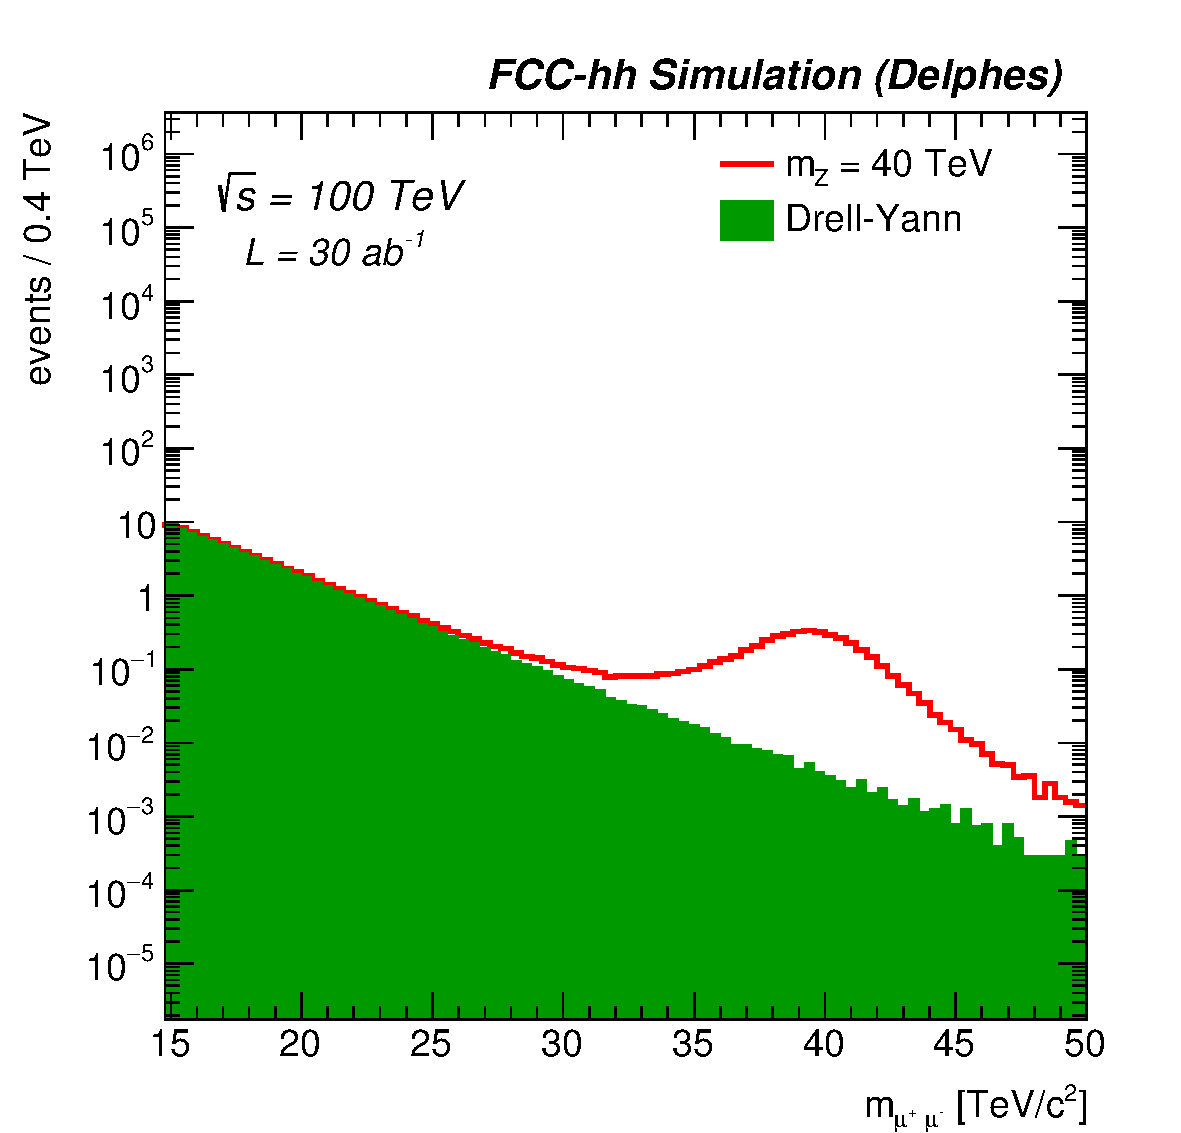
\includegraphics[width= 0.45\textwidth]{\main/experiments/img/mmumu.eps}
  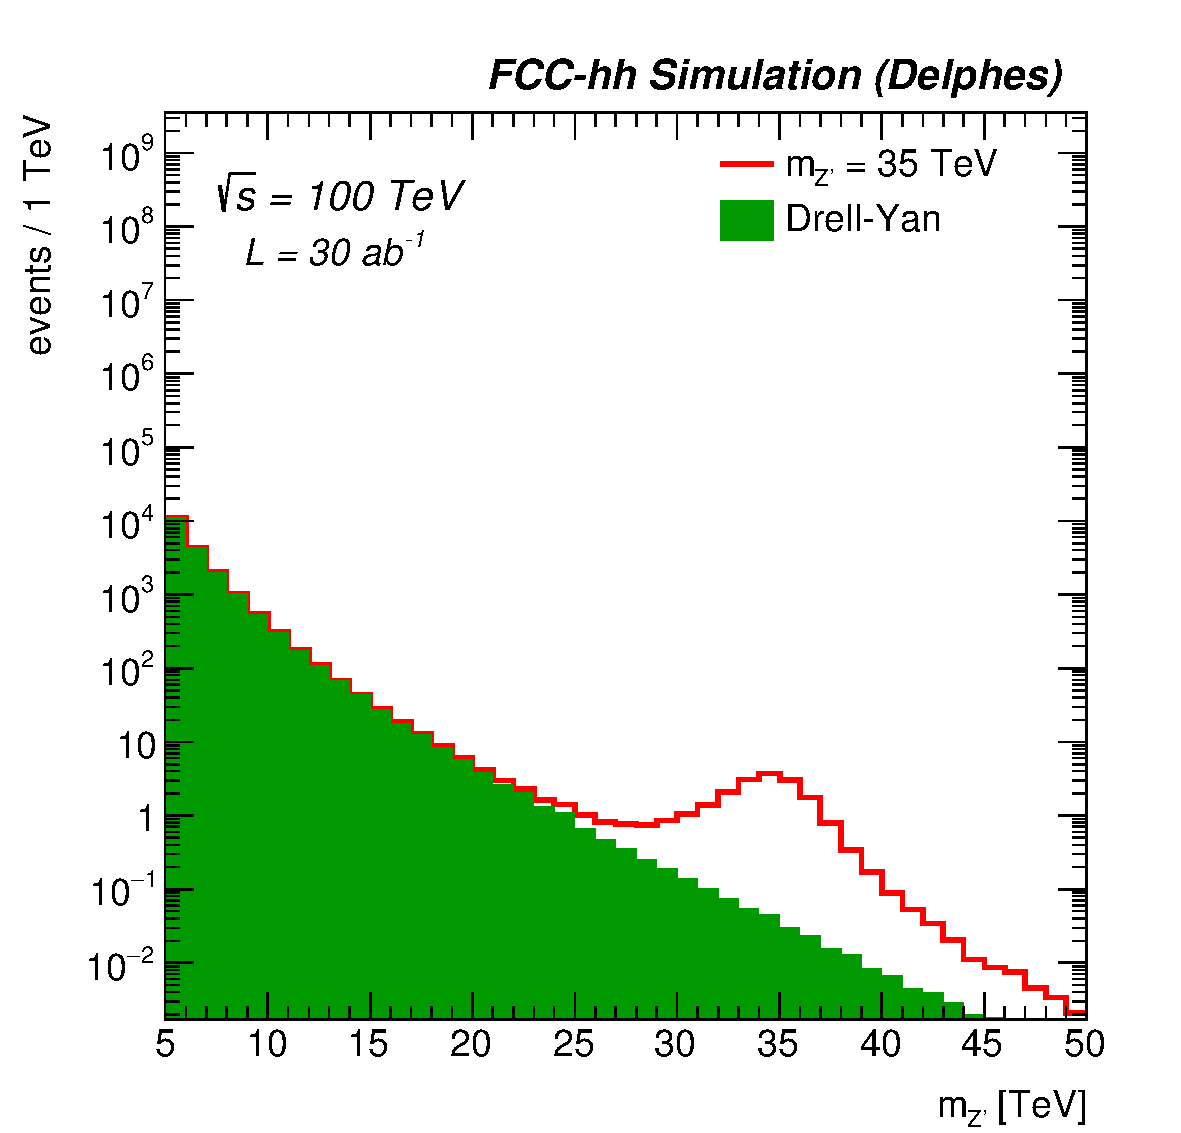
\includegraphics[width= 0.45\textwidth]{mzp_sel0_stack_log.pdf}
  %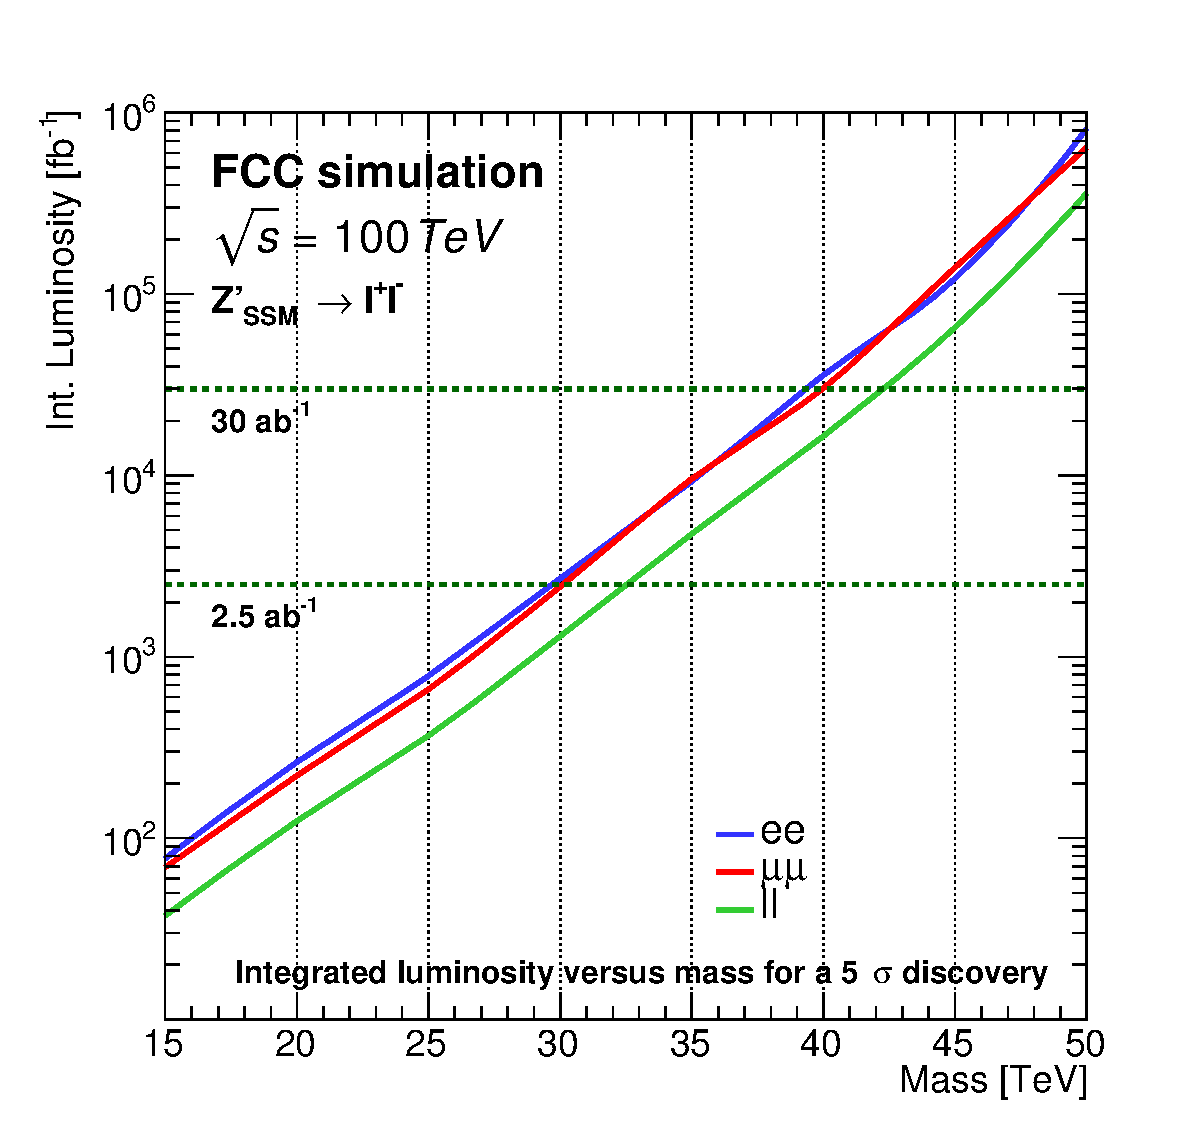
\includegraphics[width= 0.45\textwidth]{\main/experiments/img/disc-zp.eps}
  \includegraphics[width= 0.45\textwidth]{DiscoveryPotential_ll_comb_rootStyle.eps}
  \caption{Left: he di-muon invariant mass spectrum for a signal of $m_{\rm Z^{\prime}} {=} 40$~TeV and background. The background is displayed with a solid histogram and the distribution of the signal model is shown with a solid red line. The expected yields are scaled to 30\,ab$^{-1}$. Right: integrated luminosity as a function of the 5$\sigma$ discovery reach for the e$^+$e$^-$, \textmu$^+$\textmu$^-$ channels and their combination.}
  \label{fig:zprime}
\end{Figure}


\subsection{Top Squarks}
Supersymmetry is a theoretical framework that can address the hierarchy problem, allows for the unification of couplings at high energies and provides a natural dark matter candidate, often the lightest neutralino.%~\cite{Miyazawa:1966mfa,Golfand:1971iw,Neveu:1971rx,Neveu:1971iv,Ramond:1971gb,Volkov:1973ix,Wess:1973kz,Wess:1974tw}. 
The scalar partner of the top quark, known as the top squark or stop, can be produced through pp$\rightarrow \tilde{\rm t} \tilde{\rm t}$, and detected via the $\rm \tilde{t} \rightarrow t + \tilde{\chi}_1^{0}$ decay mode, where $\rm \tilde{t}_{1}$ is the stop's lightest mass eigenstate and $\tilde{\chi}_1^{0}$ is the lightest neutralino.%~\cite{Dimopoulos:1981zb,Fayet:1976et,Fayet:1977yc,Fayet:1979sa,Farrar:1978xj}. 
We focus here on fully hadronic final states. These have a striking signature: the presence of two on-shell top quarks, decaying to multiple jets and b jets, and large missing transverse momentum $p_T^{\mathrm{miss}}$. At the FCC-hh, the production rate of stop pairs is sizable up to $m_{\tilde{t}} \approx 10$~TeV. For such extreme kinematics, this search is very challenging, since highly boosted top quarks will be produced in the decay of massive stop quarks, leading to jets that exhibit three extremely collimated prongs. Resolving the sub-structure inside such "top" jets is key to reject the background from QCD jets and requires excellent granularities in the tracking detectors and the calorimeters. For example, the decay products of a 5\,TeV top quark are separated by $\Delta R {=} \Delta \eta \times \Delta \phi \sim 0.05$. This number has to be compared to the angular resolution estimated at the first tracker pixel layer, given by $\sigma_{\eta \times \phi} \approx 0.005$. The ECAL (HCAL) design shown in Table~\ref{calo_table3} ensures a granularity in $\sigma_{\eta \times \phi} \approx 0.01 (0.025)$ in the barrel. As a result, the present detector design should provide the needed angular separation power to resolve such boosted signatures.

Events are selected by vetoing electrons or muons and requiring high missing transverse energy ($p_T^{\mathrm{miss}}>2$ TeV). In addition, at least two high-$p_T$ jets ($p_T > 1$ TeV) are required, of which at least one is b-tagged ($N_{\rm b} \geq 1$), and at least one top-tagged jet ($N_{\rm t} \geq 1$). A top-tagging multi-variate discriminant for QCD background discrimination based on jet substructure observables has been developed specifically for this search, by using a combination of track and calorimeter-based jet variables. It provides a working point with $\sim5\%$ mistag rate from QCD and a $\sim60\%$ top identification efficiency. The dominant SM backgrounds with intrinsic $p_T^{\mathrm{miss}}$ arise from $\rm t \bar{t}$ and $\rm t \bar{t}$V (V {=} W,Z,H) production. These backgrounds are reduced by selecting events with $|\Delta \phi({\rm t},p_T^{\mathrm{miss}})| > 0.5$.  Their contributions are estimated in dedicated control regions extrapolated to the search regions with simulation. Contributions arising from EW (e.g. V+jets), single t quark, ${\rm t \bar{t}} VV$ and $\rm t \bar{t} t \bar{t}$ processes represent much smaller backgrounds and were estimated directly from simulation.

Events are divided into categories based on $N_{\rm t}$ and $N_{\rm b}$ and the shape of $p_T^{\mathrm{miss}}$ is used as the discriminating variable. Figure~\ref{stops} shows the expected signal and background contributions in the $N_t \geq 2$ and $N_{\rm b}{=}1$ category. A simultaneous fit to signal and control regions is used to determine the exclusion potential. The right plot of Fig.~\ref{stops} shows that, with 30\,ab$^{-1}$ of integrated luminosity, top squarks with mass up to $\sim$10~TeV can be excluded if the neutralino mass is below 4~TeV. It was verified that this limit is robust against the choice of systematics scenario. A more detailed discussion of this analysis can be found in Ref.~\cite{Gouskos:2642475}.
%
%
%
\begin{Figure}
  \centering
  %\includegraphics[width= 0.45\textwidth]{\main/experiments/img/sr_1.pdf}
  \includegraphics[width= 0.45\textwidth]{sr_1.pdf}
  %\includegraphics[width= 0.45\textwidth]{\main/experiments/img/lim_30ab_comb.pdf}
  \includegraphics[width= 0.45\textwidth]{lim_30ab_comb.pdf}
  \caption{Left: the $p_T^{\mathrm{miss}}$ distribution in background and signal events with $N_{\rm t} \geq 2$ and $N_{\rm b}{=}1$. The background processes are displayed with solid histograms and the distribution of one signal model is shown with solid red line. "LL" stands for "Lost Lepton" and collects all backgrounds where a lepton was not reconstructed due to inefficiency or limited detector acceptance. The expected yields are scaled to 30\,ab$^{-1}$. Right: exclusion potential for 30\,ab$^{-1}$, and the $\pm 1\sigma$ contours for the nominal systematic uncertainties.}
  \label{stops}
\end{Figure}

\subsection{Disappearing Tracks}
The simple and most minimal way to add a Dark Matter candidate to the SM consists in adding an SU(2) multiplet that contains a neutral state. In supersymmetry Higgsinos and winos represent, respectively a doublet and a triplet. If DM is the neutral wino~(higgsino) and was produced in thermal equilibrium, the upper limit on its mass is determined by the observed DM relic abundance: 3~TeV for the wino LSP scenario and 1~TeV for the higgsino LSP scenario. The FCC-hh provides therefore a unique opportunity to probe wino and higgsino DM.

When a pure wino/higgsino is the LSP, the mass of the \ensuremath{\tilde{\chi}_{1}^{0}}~is highly degenerate with the lightest chargino~(\ensuremath{\tilde{\chi}_{1}^{\pm}})~\cite{Ibe:2012sx,Thomas:1998wy}.
Therefore, \ensuremath{\tilde{\chi}_{1}^{\pm}}~is a long-lived state with a lifetime $\tau_{\chi}\approx 0.2~(0.023)$~ns for a 3~TeV wino~(1~TeV higgsino)~\cite{Barr:2002ex}.
A \ensuremath{\tilde{\chi}_{1}^{\pm}}~decays into a \ensuremath{\tilde{\chi}_{1}^{0}} and a soft charged pion. The neutralino does not interact with the detector and the pion is too soft to be reconstructed. Therefore, the long-lived chargino can be detected as a short-distance \emph{disappearing track} with a typical length scale of $\cal{O}$(1-10)\,cm~\cite{Chen:1996ap,Chen:1999yf,Asai:2008sk}.

The backgrounds for this search can be categorized into two components.
\emph{Physical} backgrounds arise from charged particles (electrons or charged pions) scattered by the material in the inner tracker. These are mainly W($\rightarrow \ell$\textnu)+jets events, with large $E_T^{\mathrm{miss}}$~and a high $p_{T}$ track from a W decay product. The normalization of the physical background is derived by taking the background rate estimated at ATLAS, and rescaling it by the ratio of the amount of the material in the FCC tracker to that in the ATLAS inner tracker. The \emph{unphysical} background consists of fake tracks; they arise from a random combination of hits that form a short track. The fake-track rate is evaluated from simulated minimum bias events by counting the number of fake tracks passing the quality requirements. The final estimate is obtained by scaling by a pile-up dependent fake rate probability. A good coverage of the volume within r~$<$~10~cm is crucial for an optimal fake-track rejection and thus for the success of this measurement.

Candidate events are required to contain at least one high $p_{T}$ jet, large \ensuremath{p_{T}^{\rm{miss}}} and no lepton~(electron or muon) with $p_{T}$ above 10~GeV.
The jet $p_{T}$ and \ensuremath{p_{T}^{\rm{miss}}}~thresholds are determined by maximizing the sensitivity at each \ensuremath{\tilde{\chi}_{1}^{\pm}}~mass point based on the signal acceptance and background rate. Additionally, at least one short track with \ensuremath{N_{\mathrm{layer}}^{\mathrm{hit}}}\,$\geq$\,5 is required.

The expected significance obtained with the default tracker layout (described in Section 7.5.1 \MS{fix by linking to actual figure}) is shown in Figure~\ref{figure:SignificanceEta1} as the grey band.  The area represents an estimate of the uncertainty obtained from different QCD models of pile-up simulation. The impact of a layout with 5 pixels tracking layers instead of 4 is shown in red. Two pile-up conditions, $\left< \mu \right>$ {=} 200 and 500, have been considered to evaluate the fake-tracks background. A significance well above 5$\sigma$ for the 3~TeV wino can be reached. However, a 5$\sigma$ significance for the 1~TeV higgsino can be reached only using the alternative layout with 5 pixel layers. The sensitivity could be further improved by using the hit-timing information to suppress fake tracks or using dE/dx information to identify the velocity of the disappearing track.

\begin{Figure}
  \centering
  %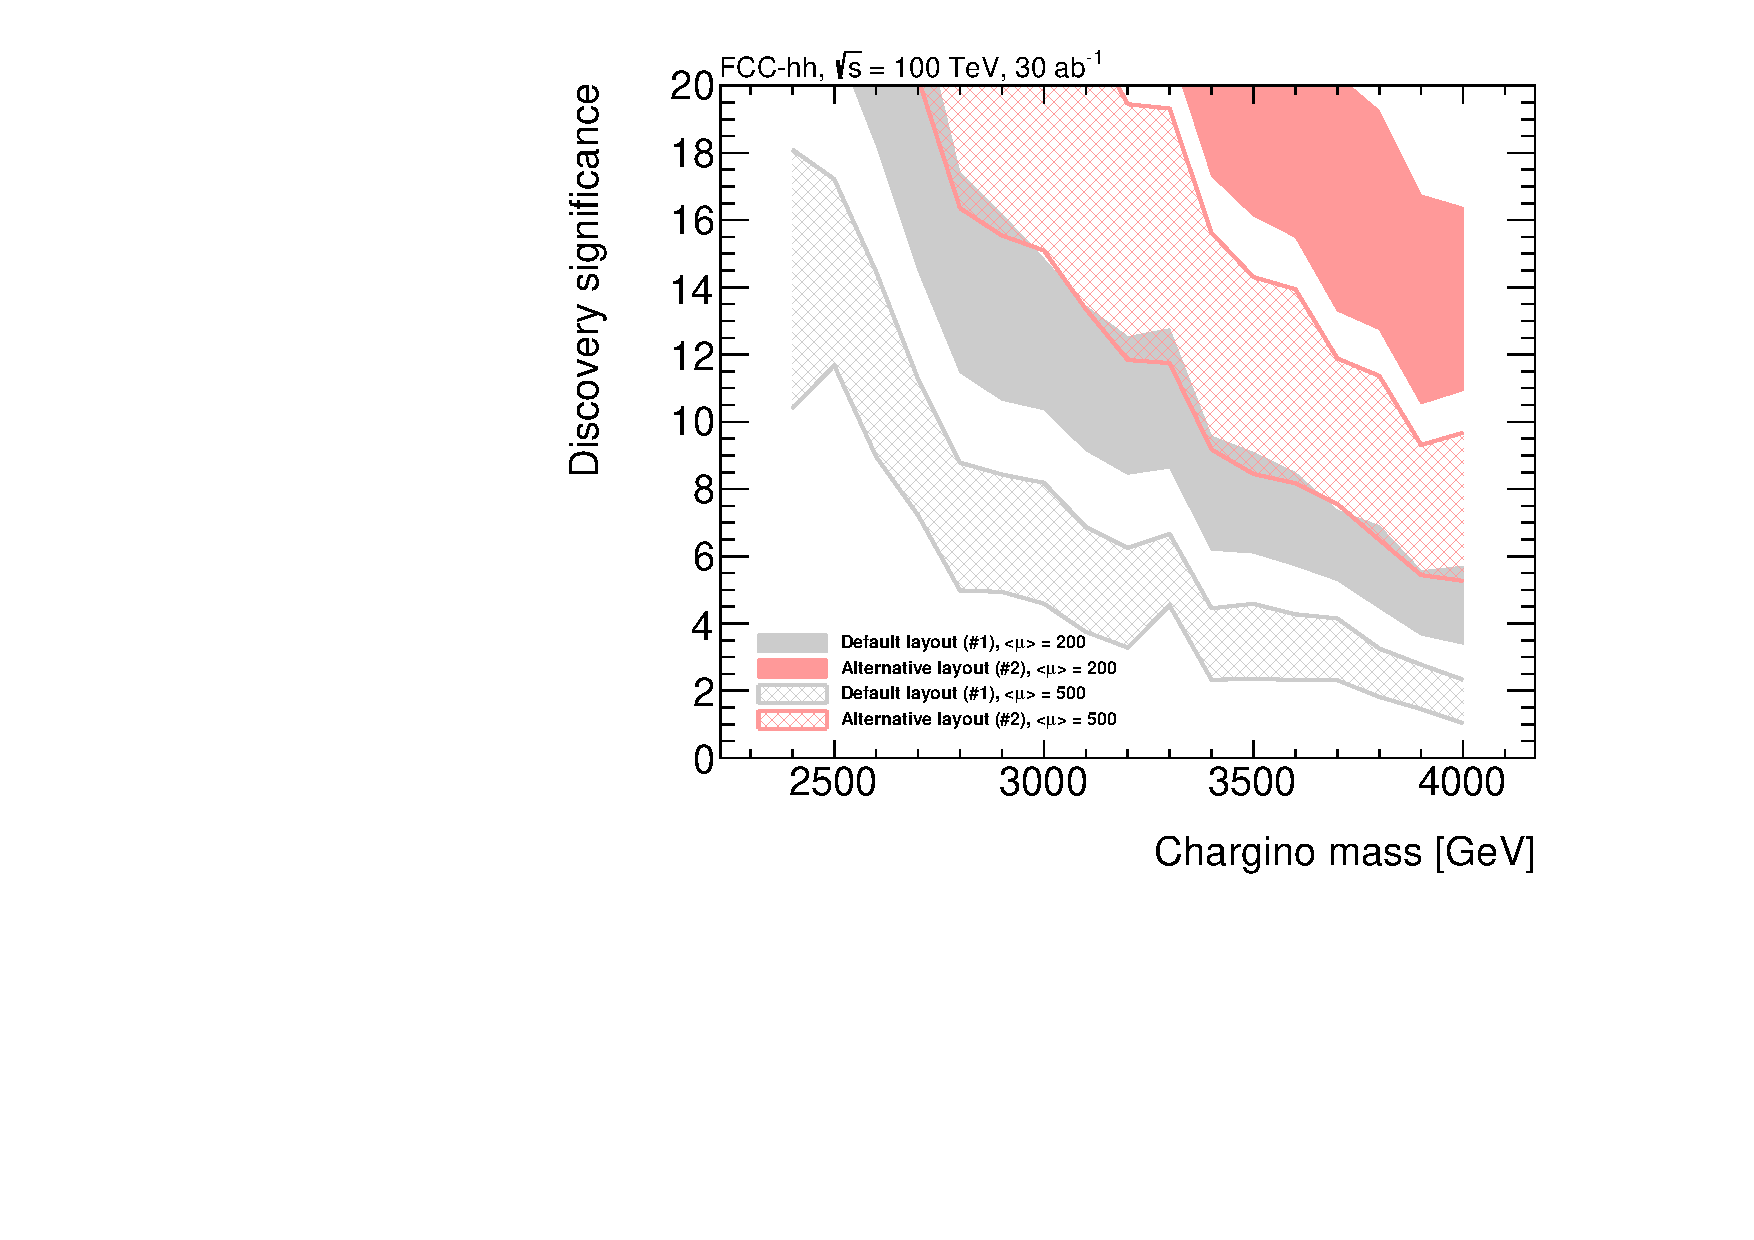
\includegraphics[width=0.48\textwidth]{\main/experiments/img/h_Significance_di_wino9_eta.pdf}
  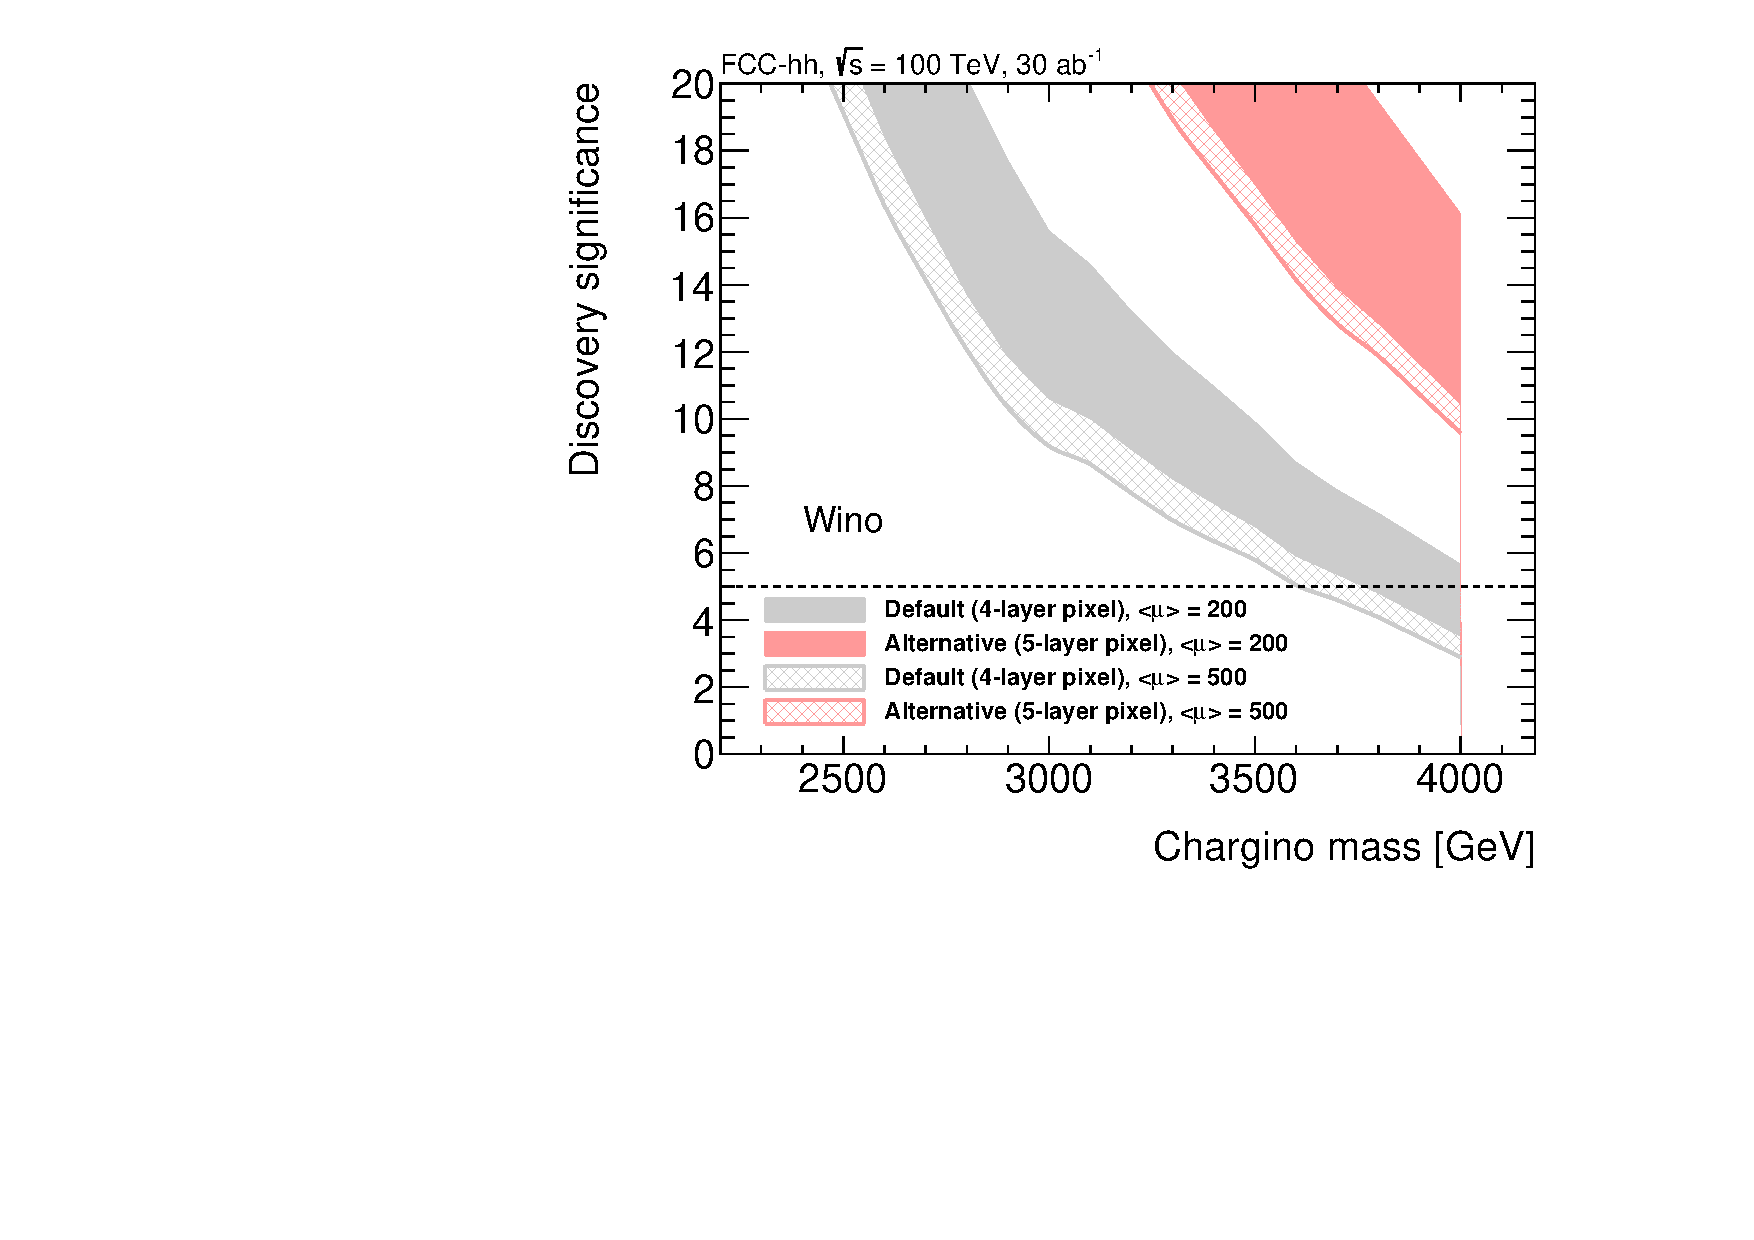
\includegraphics[width=0.48\textwidth]{h_Significance_wino12_eta_5hits.pdf}
  %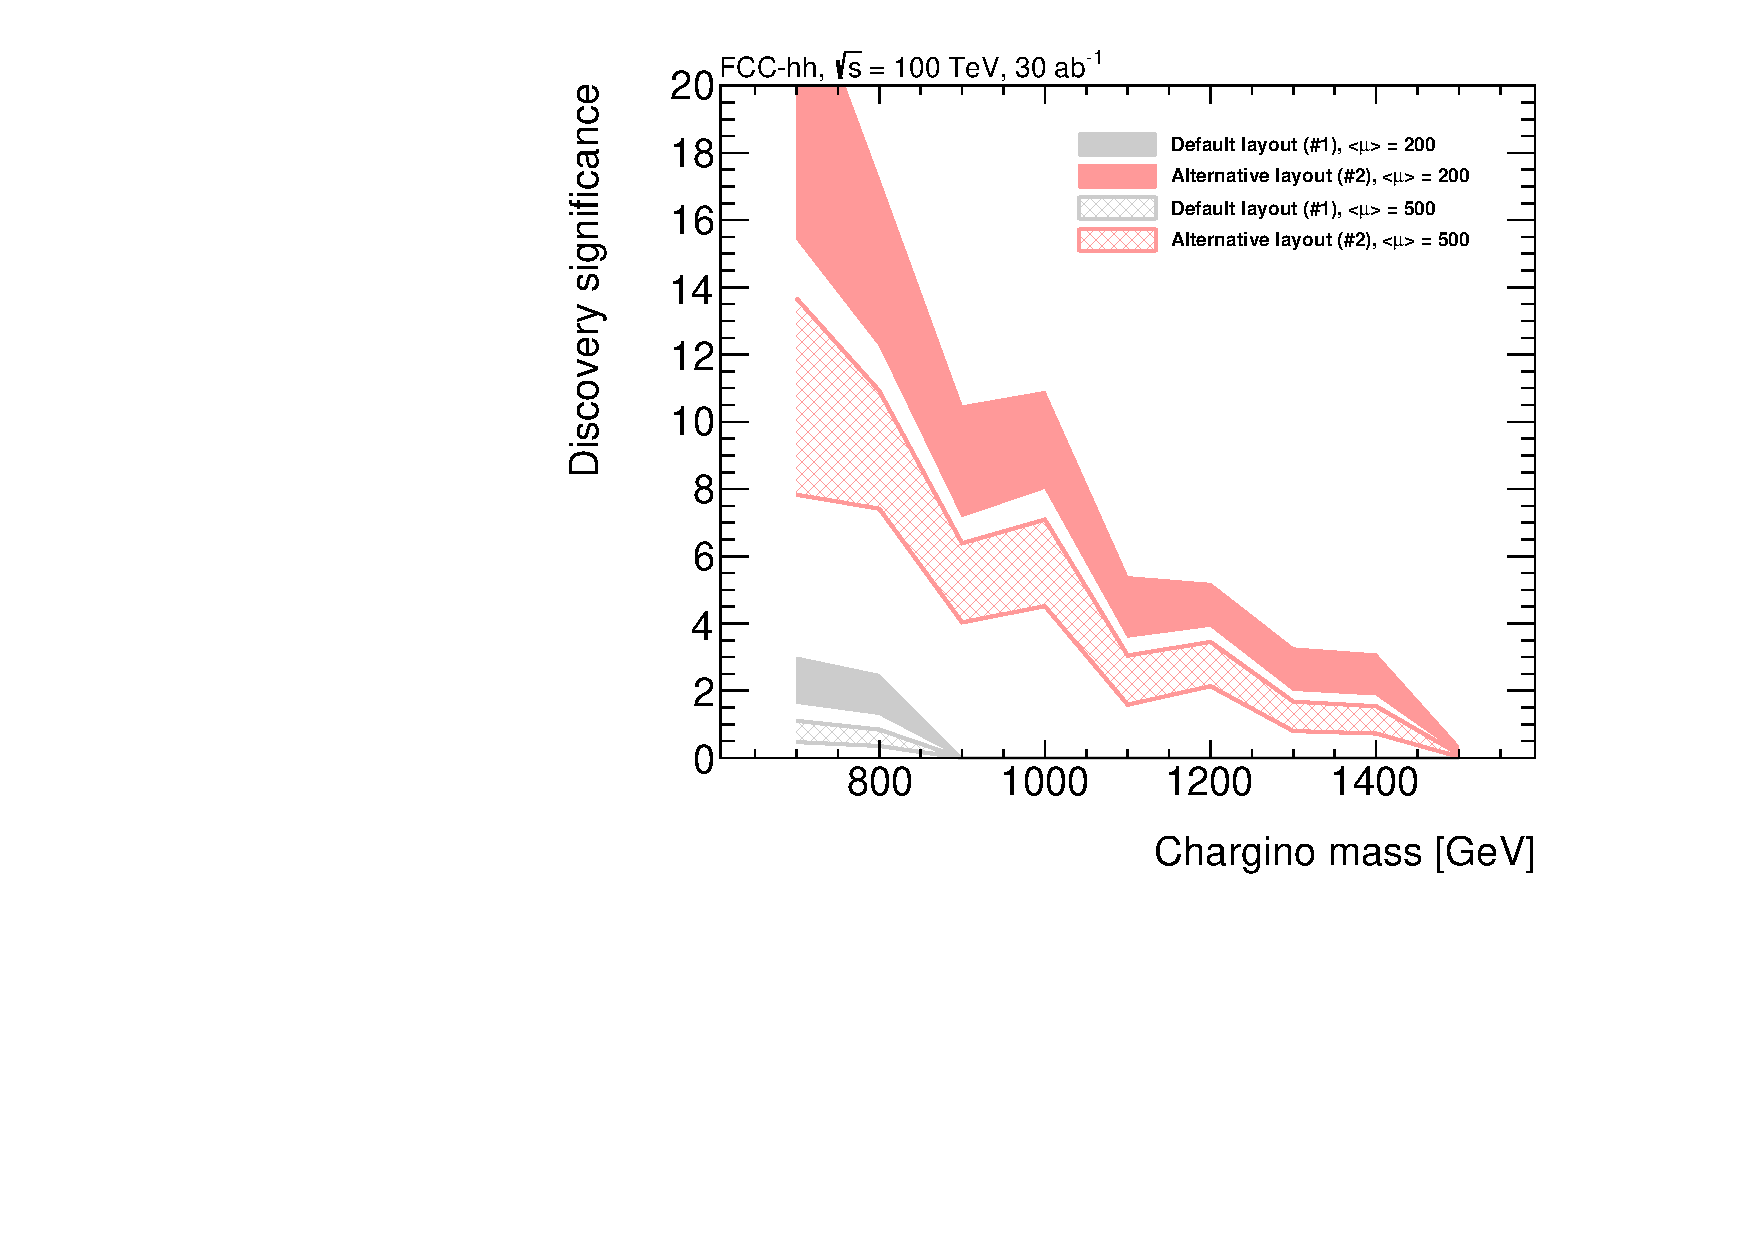
\includegraphics[width=0.48\textwidth]{\main/experiments/img/h_Significance_di_higgsino9_eta.pdf}
  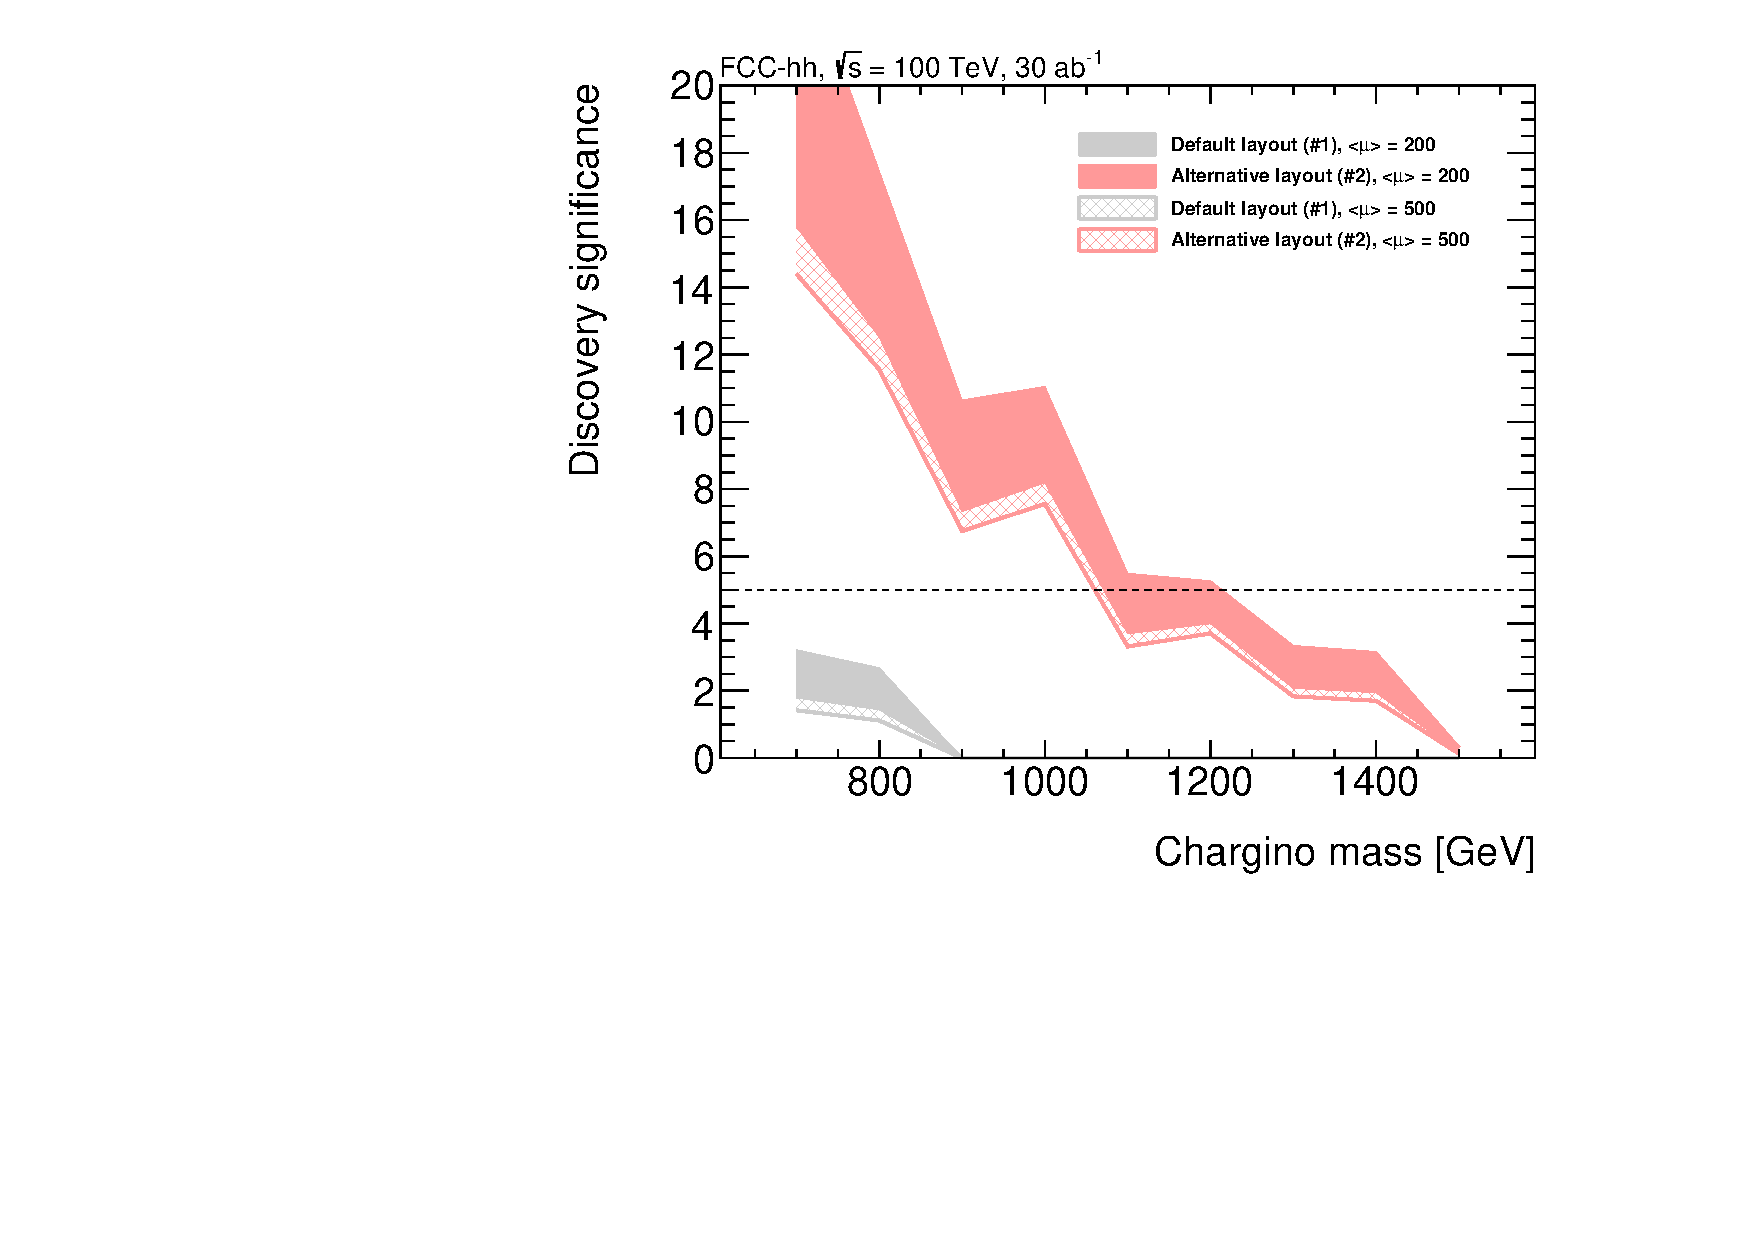
\includegraphics[width=0.48\textwidth]{h_Significance_higgsino12_eta_5hits.pdf}
  \caption{Left: wino, $\left< \mu\right>$ {=} 500. Right: higgsino, $\left< \mu\right>$ {=} 200. Expected discovery significance at 30\,ab${}^{-1}$ with requirements of \ensuremath{N_{\mathrm{layer}}^{\mathrm{hit}}}~$\geq$ 5 with 200 (solid) or 500 (hatched) pile-up collisions and $|\eta|<$ 1 with the default (grey) and alternative (red) layouts.
            The band width corresponds to the difference of the two configurations of the soft QCD processes.}
  \label{figure:SignificanceEta1}
\end{Figure}

\bibliographystyle{fcc}
\bibliography{bibliography.bib}
\end{document}